\documentclass[a4paper,12pt]{report}
\usepackage[T1]{fontenc}
\usepackage{lmodern}
\usepackage{amsmath}
\usepackage{amsfonts}
\usepackage{amssymb}
\usepackage{amsthm}
\usepackage{graphicx}
\usepackage{hyperref}
\usepackage{color}
\usepackage{xcolor}
\usepackage{url}
\usepackage{textcomp}
\usepackage{listings}

\title{Písemná práce}
\author{\parbox{\linewidth}{\center%
Vojtech Vasek\endgraf\bigskip
E2A\endgraf}}
\date{\today}

\begin{document}

\maketitle
\tableofcontents
\newpage
\chapter{Apple představil M2 Pro a M2 Max}
\begin{figure}[htp]
\centering
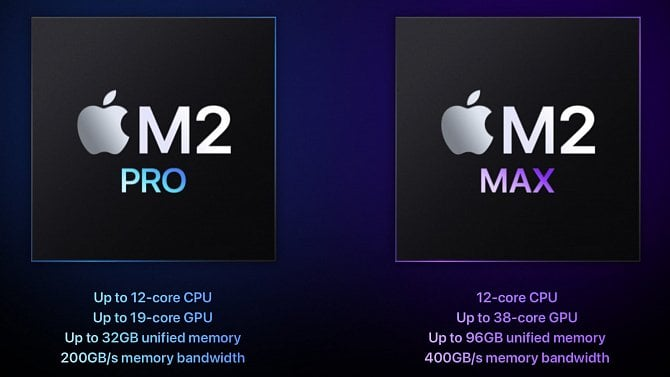
\includegraphics[width=8cm]{IKT_18_1_23@2.jpg}
\caption{Autor: Apple}
\end{figure}
Na dříve uvedený model M2, první z druhé generace velkých ARM SoC pro plnohodnotné počítače nyní Apple navazuje dvěma vyššími modely. M2 Pro dostal 12jádrové CPU a 19jádrové GPU s podporou až 32 GB unifikované RAM s propustností 200 GB/s. Model M2 Max pak nabízí stejnou CPU část, k ní však 38jádrové GPU a podporu až 96 GB RAM s propustností 400 GB/s.

I tyto nové procesory jsou samozřejmě vyráběny 5nm procesem u TSMC, model Pro nese 40 miliard tranzistorů, model Max 67 miliard. V obou případech, stejně jako u M2 versus M1, jde o solidní nárůst parametrů ve srovnání s první generací, tedy zde s modely M1 Pro / Max. Uvidíme, kdy a jestli Apple přijde i s nejvyšším modelem M2 Ultra.

Nové procesory jsou základem nových modelů notebooků MacBook Pro a také minipočítačů mac Mini.
\chapter{Linuxové prohlížeče dokumentů zvládnou české znaky v PDF formulářích}
\begin{figure}[htp]
\centering

\includegraphics[width=16cm]{IKT_18_1_23@3.jpg}
\caption[ ]{Autor: www.shutterstock.com, podle licence: Rights Managed}
\end{figure}
Adobe odřízlo linuxové uživatele už před deseti lety a od té doby jsme odkázaní na svobodné prohlížeče dokumentů. Ty fungují dobře, ale při vyplňování formulářů mají velké problémy s českými znaky. "Je to způsobené tím, že samotný standard PDF zná jen základní sady znaků, v kterých znaky české abecedy chybí," vysvětluje Jiří Eischmann na blogu Fedora.cz. Standard sice zná ještě znakovou sadu RTF, ale ta zase není podporovaná všemi klienty. "Najít tedy řešení nad rámec standardu, které bude kompatibilní napříč různými implementacemi, není jednoduchá záležitost."

Dobrou zprávou je, že se vývojářům podařilo do renderovací knihovny poppler doplnit podporu pro unicode pomocí přikládání písma, které tuto znakovou sadu podporuje, k danému dokumentu. To znamená, že všechny aplikace, které tuto knihovnu využívají, budou moci správně sloužit k vyplňování českých formulářů v PDF.

Týká se to například populárních prohlížeček Evince nebo Okular. Změna už byla backportována do Fedory 37 a časem se dostane i do dalších distribucí.
\newpage
\chapter[Volume Levels]{\#78 Volume Levels}
\section{Core Apps and Libraries}
\subsection{Settings}
The redesign of the sound panel of GNOME Settings is continuing! This week the “Volume Levels” section has been moved in a separate window, to make the main panel more compact by default. Also, the app icons in the new design are now bigger and full-colored and the rows also include a volume level indicator.
\begin{figure}[htp]
\centering
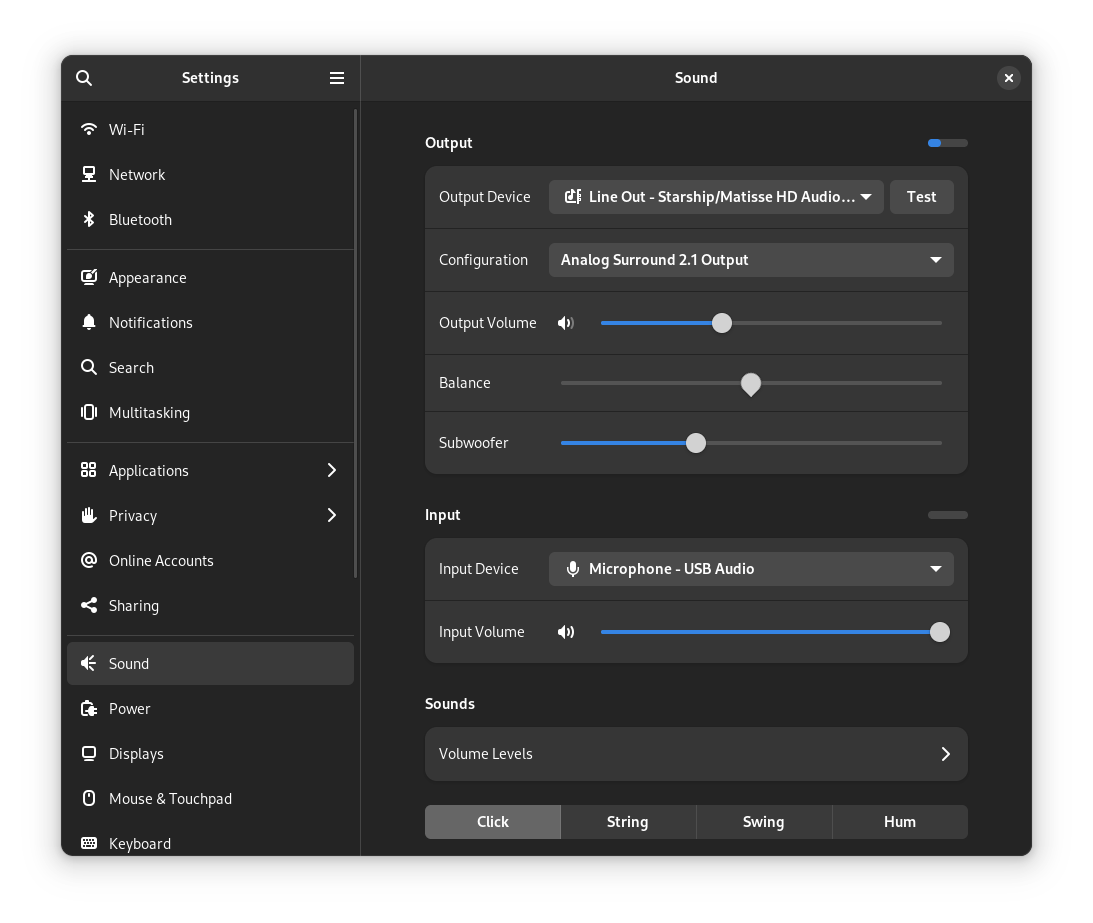
\includegraphics[width=8cm]{IKT_18_1_23@4.png}
\end{figure}
\begin{figure}[htp]
\centering
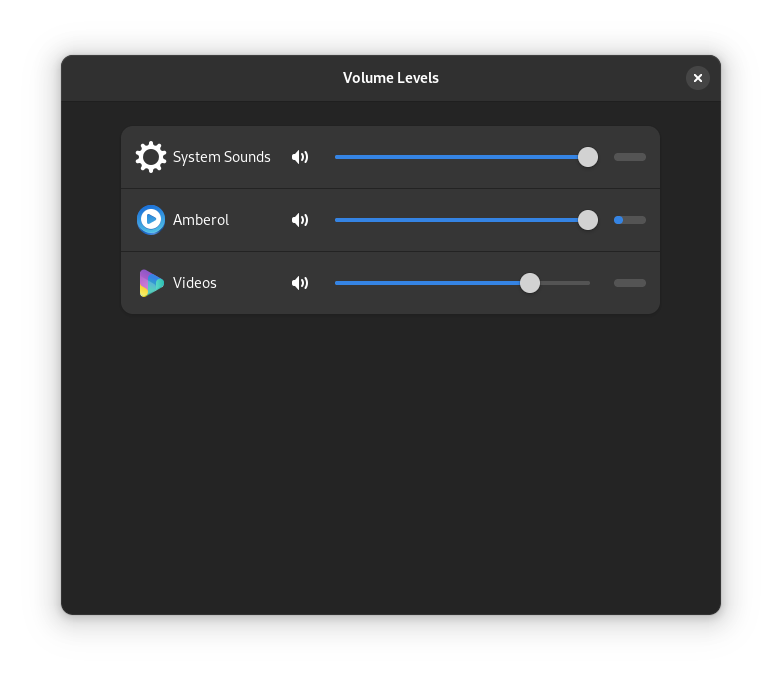
\includegraphics[width=8cm]{IKT_18_1_23@5.png}
\end{figure}
\section{Circle Apps and Libraries}
\subsection{Gaphor}
This week Dan Yeaw released Gaphor 2.15.0. The improvements include, but are not limited to:

\begin{itemize}
\item Basic git merge conflict support by asking which model to load
\item Improvements to CSS autocomplete for Gaphor’s style sheets
\item Native file chooser support in Windows
\item Fixed UTF-8 encoding issues on Windows
\item Fixed translations not loading in Windows, macOS, and AppImage
\end{itemize}
Many thanks to everyone who helped out with translating Gaphor. Special thanks for Jonathan and Óscar Fernández Díaz for their code contributions.
\begin{figure}[htp]
\centering
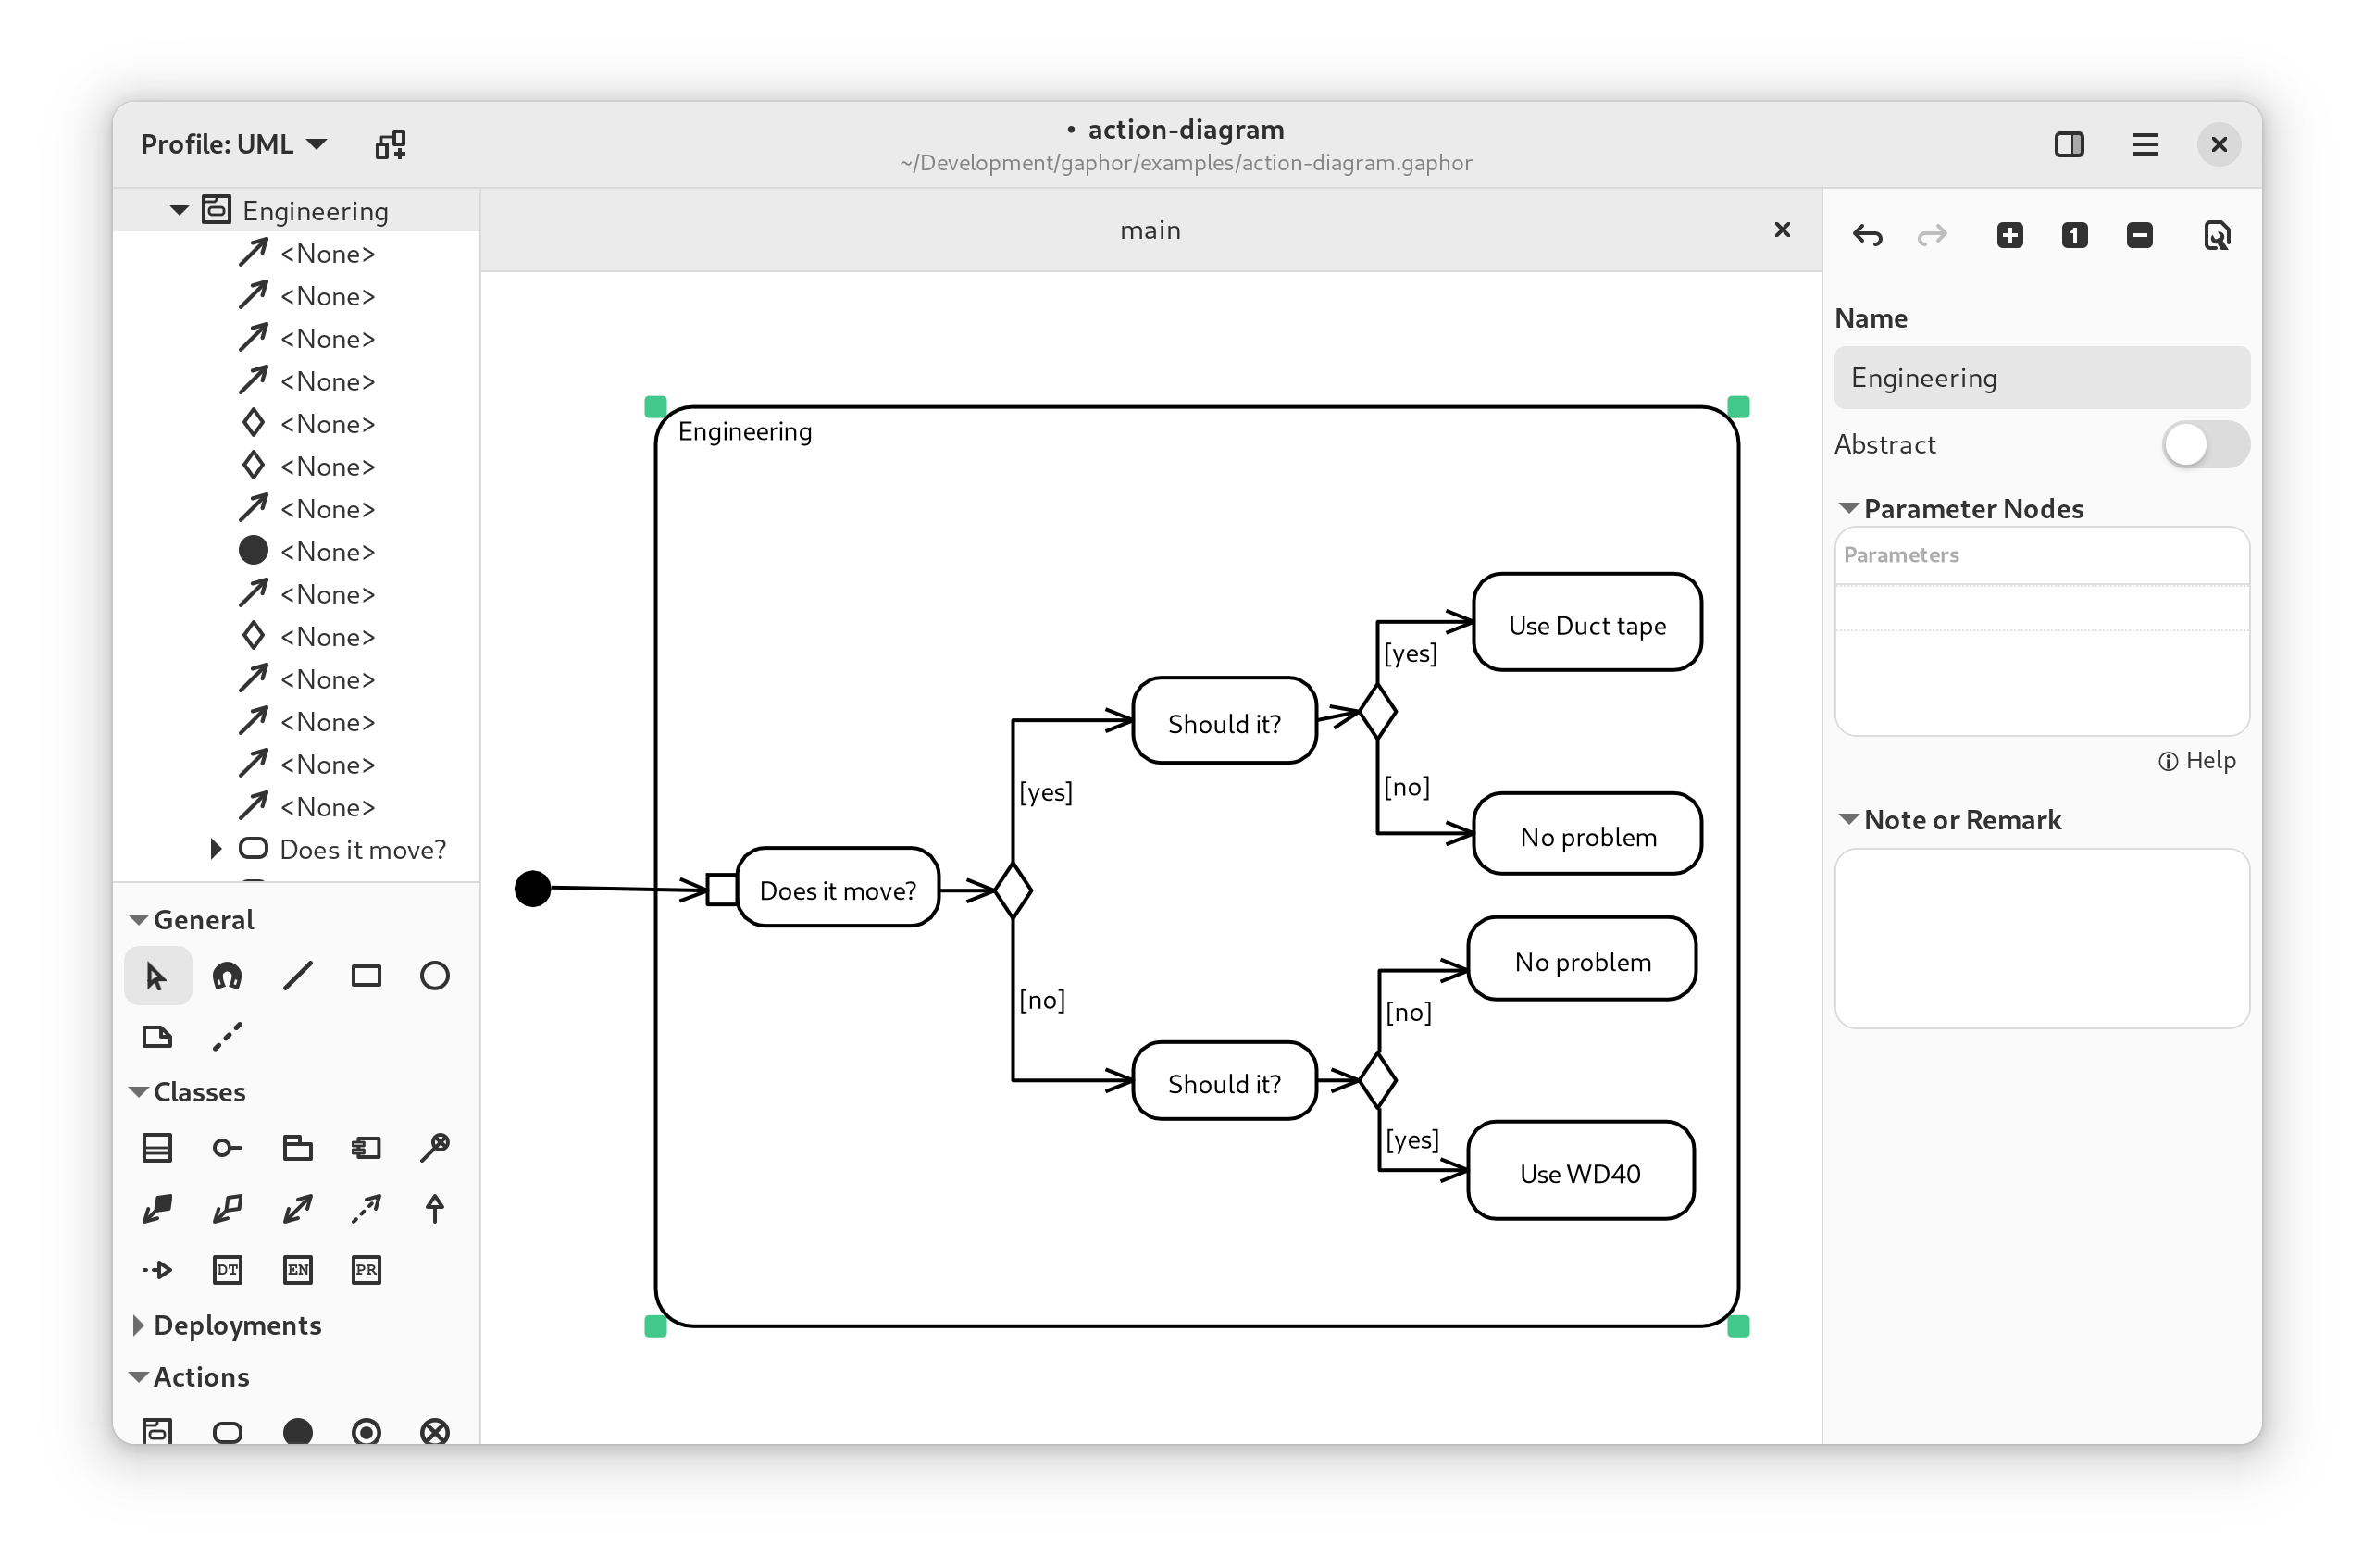
\includegraphics[width=8cm]{IKT_18_1_23@6.png}
\end{figure}
\section{Third Party Projects}
Black Box 0.13.0 is finally out! This release brings much-anticipated features and bug fixes:
\begin{itemize}
\item Customizable keyboard shortcuts with support for fully disabling shortcuts
\item Background transparency
\item Customizable cursor blinking mode
\item Experimental Sixel support (Settings > Advanced > Sixel Support)
\item Fixed scrolling on touchpad and touchscreens
\item Fixed issues with copy/paste
\end{itemize}
You can check out the full release notes \href{https://gitlab.gnome.org/raggesilver/blackbox/-/releases/v0.13.0}{here}


\subsection{Rnote}
I just merged the \verb|tabs| branch into \verb|main| in the Rnote repository. Thanks to the awesome “TabView” libadwaita widget the tabs themselves were really easy to implement. Alongside with it I also implemented a global colorpicker, and made the UI more pretty with floating toolbars. There are still some things left to do and likely bugs to squash, but I am really excited to get this out as a beta release soon.

\chapter{Tabulka a průměry}

\begin{tabular}{|l|c|c|c|r|}
\hline
\# & A & B & C & D \\
\hline
0 & 0 & 0 & 0 & 0 \\
\hline
1 & 0 & 0 & 0 & 1 \\
\hline
2 & 0 & 0 & 1 & 0 \\
\hline
3 & 0 & 0 & 1 & 1 \\
\hline
4 & 0 & 1 & 0 & 0 \\
\hline
5 & 0 & 1 & 0 & 1 \\
\hline
6 & 0 & 1 & 1 & 0 \\
\hline
7 & 0 & 1 & 1 & 1 \\
\hline
8 & 1 & 0 & 0 & 0 \\
\hline
9 & 1 & 0 & 0 & 1 \\
\hline
A & 1 & 0 & 1 & 0 \\
\hline
B & 1 & 0 & 1 & 1 \\
\hline
C & 1 & 1 & 0 & 0 \\
\hline
D & 1 & 1 & 0 & 1 \\
\hline
E & 1 & 1 & 1 & 0 \\
\hline
F & 1 & 1 & 1 & 1 \\
\hline
\end{tabular}


${\bar {x}}={\frac {1}{n}}\left(x_{1}+x_{2}+\ldots +x_{n}\right)={\frac {1}{n}}\sum _{{i=1}}^{{n}}x_{i}$

$G(x_1,x_2,...,x_n) = \sqrt[n]{x_1*x_2***x_n} = (\prod_{i=1}^{n} x_i)^{1/n}$
\end{document}